\documentclass[11pt,a4paper]{article}

\usepackage[utf8]{inputenc}
\usepackage[english]{babel}
\usepackage[T1]{fontenc}

\usepackage{amsmath,amssymb,amsfonts}

\usepackage{hyperref}
\usepackage{graphicx}

\title{Computational Geometry - Point Location}
\author{Philip Munksgaard \\ Sebastian Paaske Tørholm \\ Ejnar Håkonsen}

\begin{document}
\maketitle

\section{Exercise 6.5}

Given an convex polygon $\mathcal{P}$ as an array of its $n$ vertices
in sorted order around the boundary, we wish to decide in $O(\log n)$
time whether a query point $q$ is inside the polygon.

We do this by a recursive binary search. Find the point in the middle
of the array, and determine whether or not the angle $\angle p_1
p_{n/2} q$ is a left turn or a right turn. If it is a left turn,
recursively go into the left half of the array (still using $p_1$ as
the origin point) and similarly for right turns. If at some point we
only have three points (and thus a triangle), checking whether $q$ is
inside that triangle is a constant time operation. Since we always
half the amount of vertices in our array, we are guaranteed to reach
the base case at some point, and we only use $O(\log n)$ time.

\section{Exercise 6.6}
Given a y-monotone polygon $\mathcal{P}$ as an array of its $n$ vertices
in sorted order around the boundary, we wish to decide in $O(\log n)$
time whether a query point $q$ is inside the polygon.

First we find the topmost and bottommost points $p_t$ and $p_b$ using binary
search on the polygon. On both sides, we now use binary search to locate the
points with y-coordinate immediately above ($p_{lu}$ and $p_{ru}$) and below
($p_{lb}$ and $p_{rb}$) $q$.

If $q$ is in $\mathcal{P}$, $q$ must be contained within the convex polygon
$(p_{lu}, p_{ru}, p_{rb}, p_{lb})$. Checking if the point is contained
within this can be done in constant time.

\section{Exercise 6.7}

Here, we can extend the algorithm from exercise 6.5. However, we
need to start by simplifying the problem a bit, by finding a
corresponding polygon $\mathcal{P}'$ where the point $p$ is one of the
borders. We do this by picking a point $p'$ in $\mathcal{P}$. Then we
draw and extend a line from $p$ to $p'$. Now, we can find two points
$p_i$ and $p_{i+1}$ such that they are on each side of the line
protruding from $pp'$. These points are uniquely determined due to the
star shape of $P$, and can be found in $O(\log n)$ using binary search.
\footnote{Assuming that no three points are colinear. If there exists
    a $p_i$ that is colinear with $p$ and $p'$, we can simply ignore
    $R1$ as it degenerates, and use the same method as the one outlined
    with $p_i$ in place of $p_{i+1}$.}

\begin{figure}[h!]
    \centering
    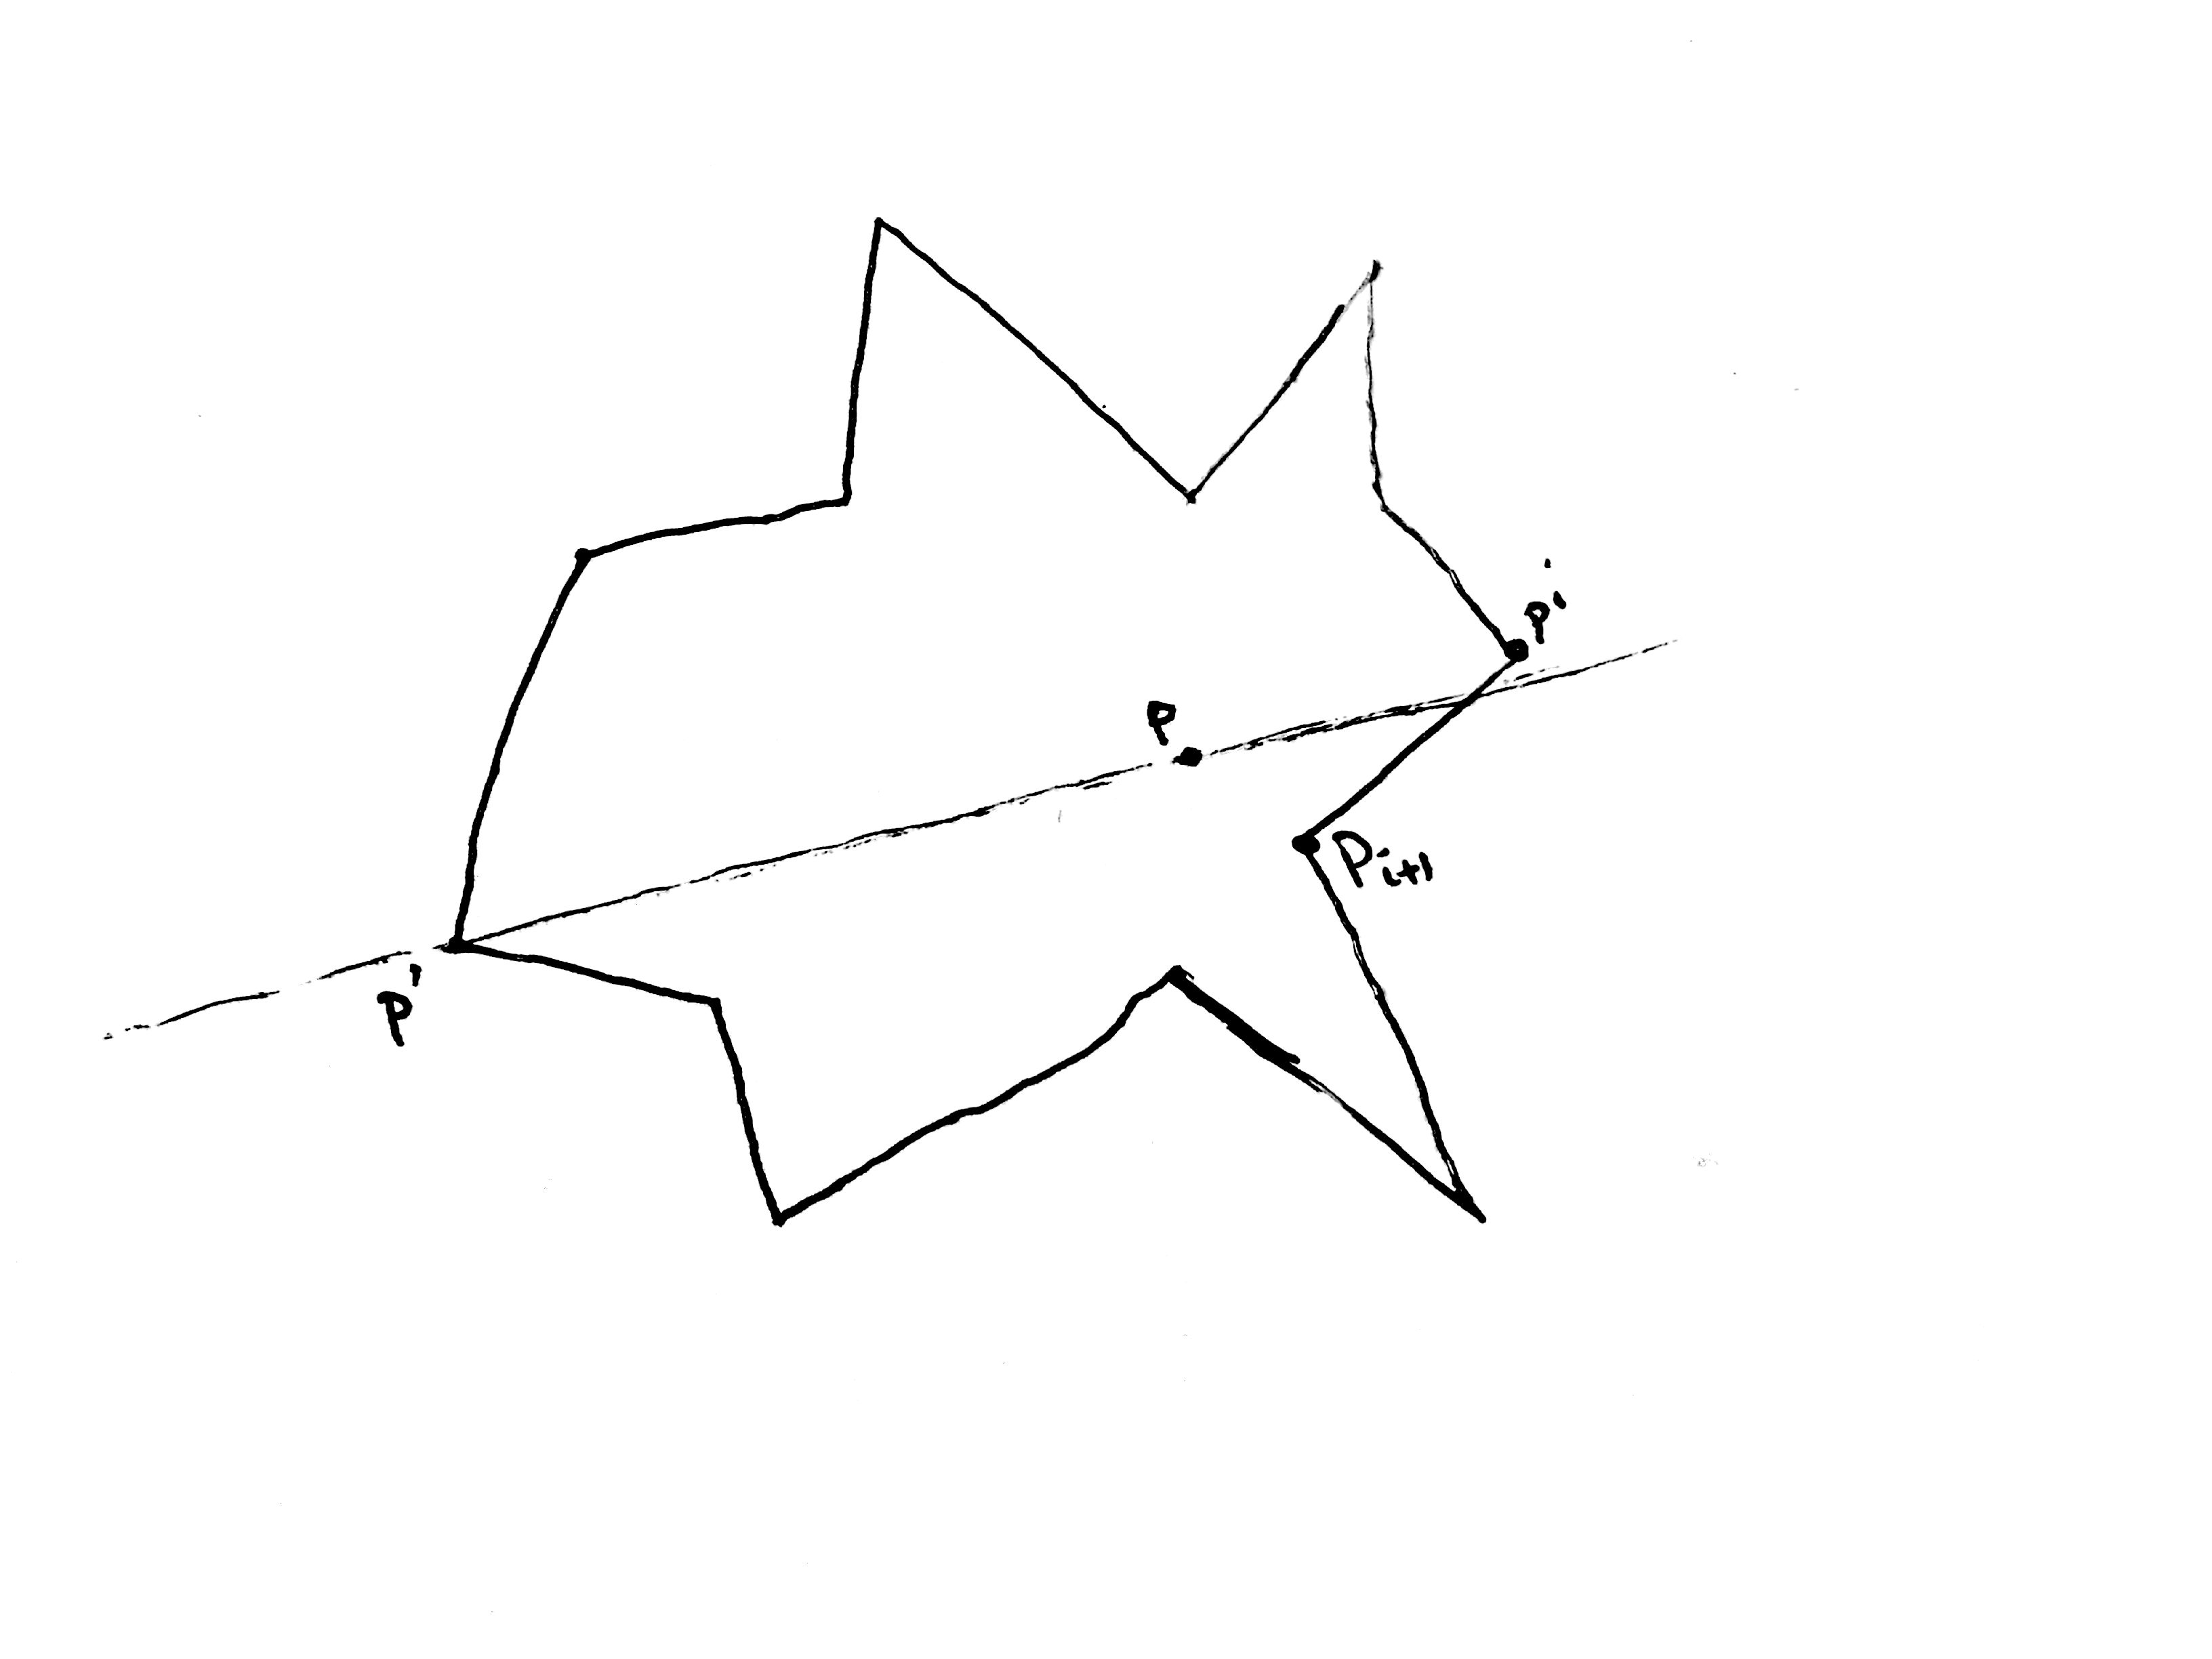
\includegraphics[width=.7\textwidth]{regionsstar1.jpg}
    \caption{Finding $p_i$ and $p_{i+1}$ in the star shaped polygon.}
\end{figure}

We now have that $q$ is contained within one of the three regions induced
by the half-lines $p p_i$, $p p_{i+1}$ and $p p'$. We name these regions
as shown in \autoref{regions-star}.

\begin{figure}[h!]
    \centering
    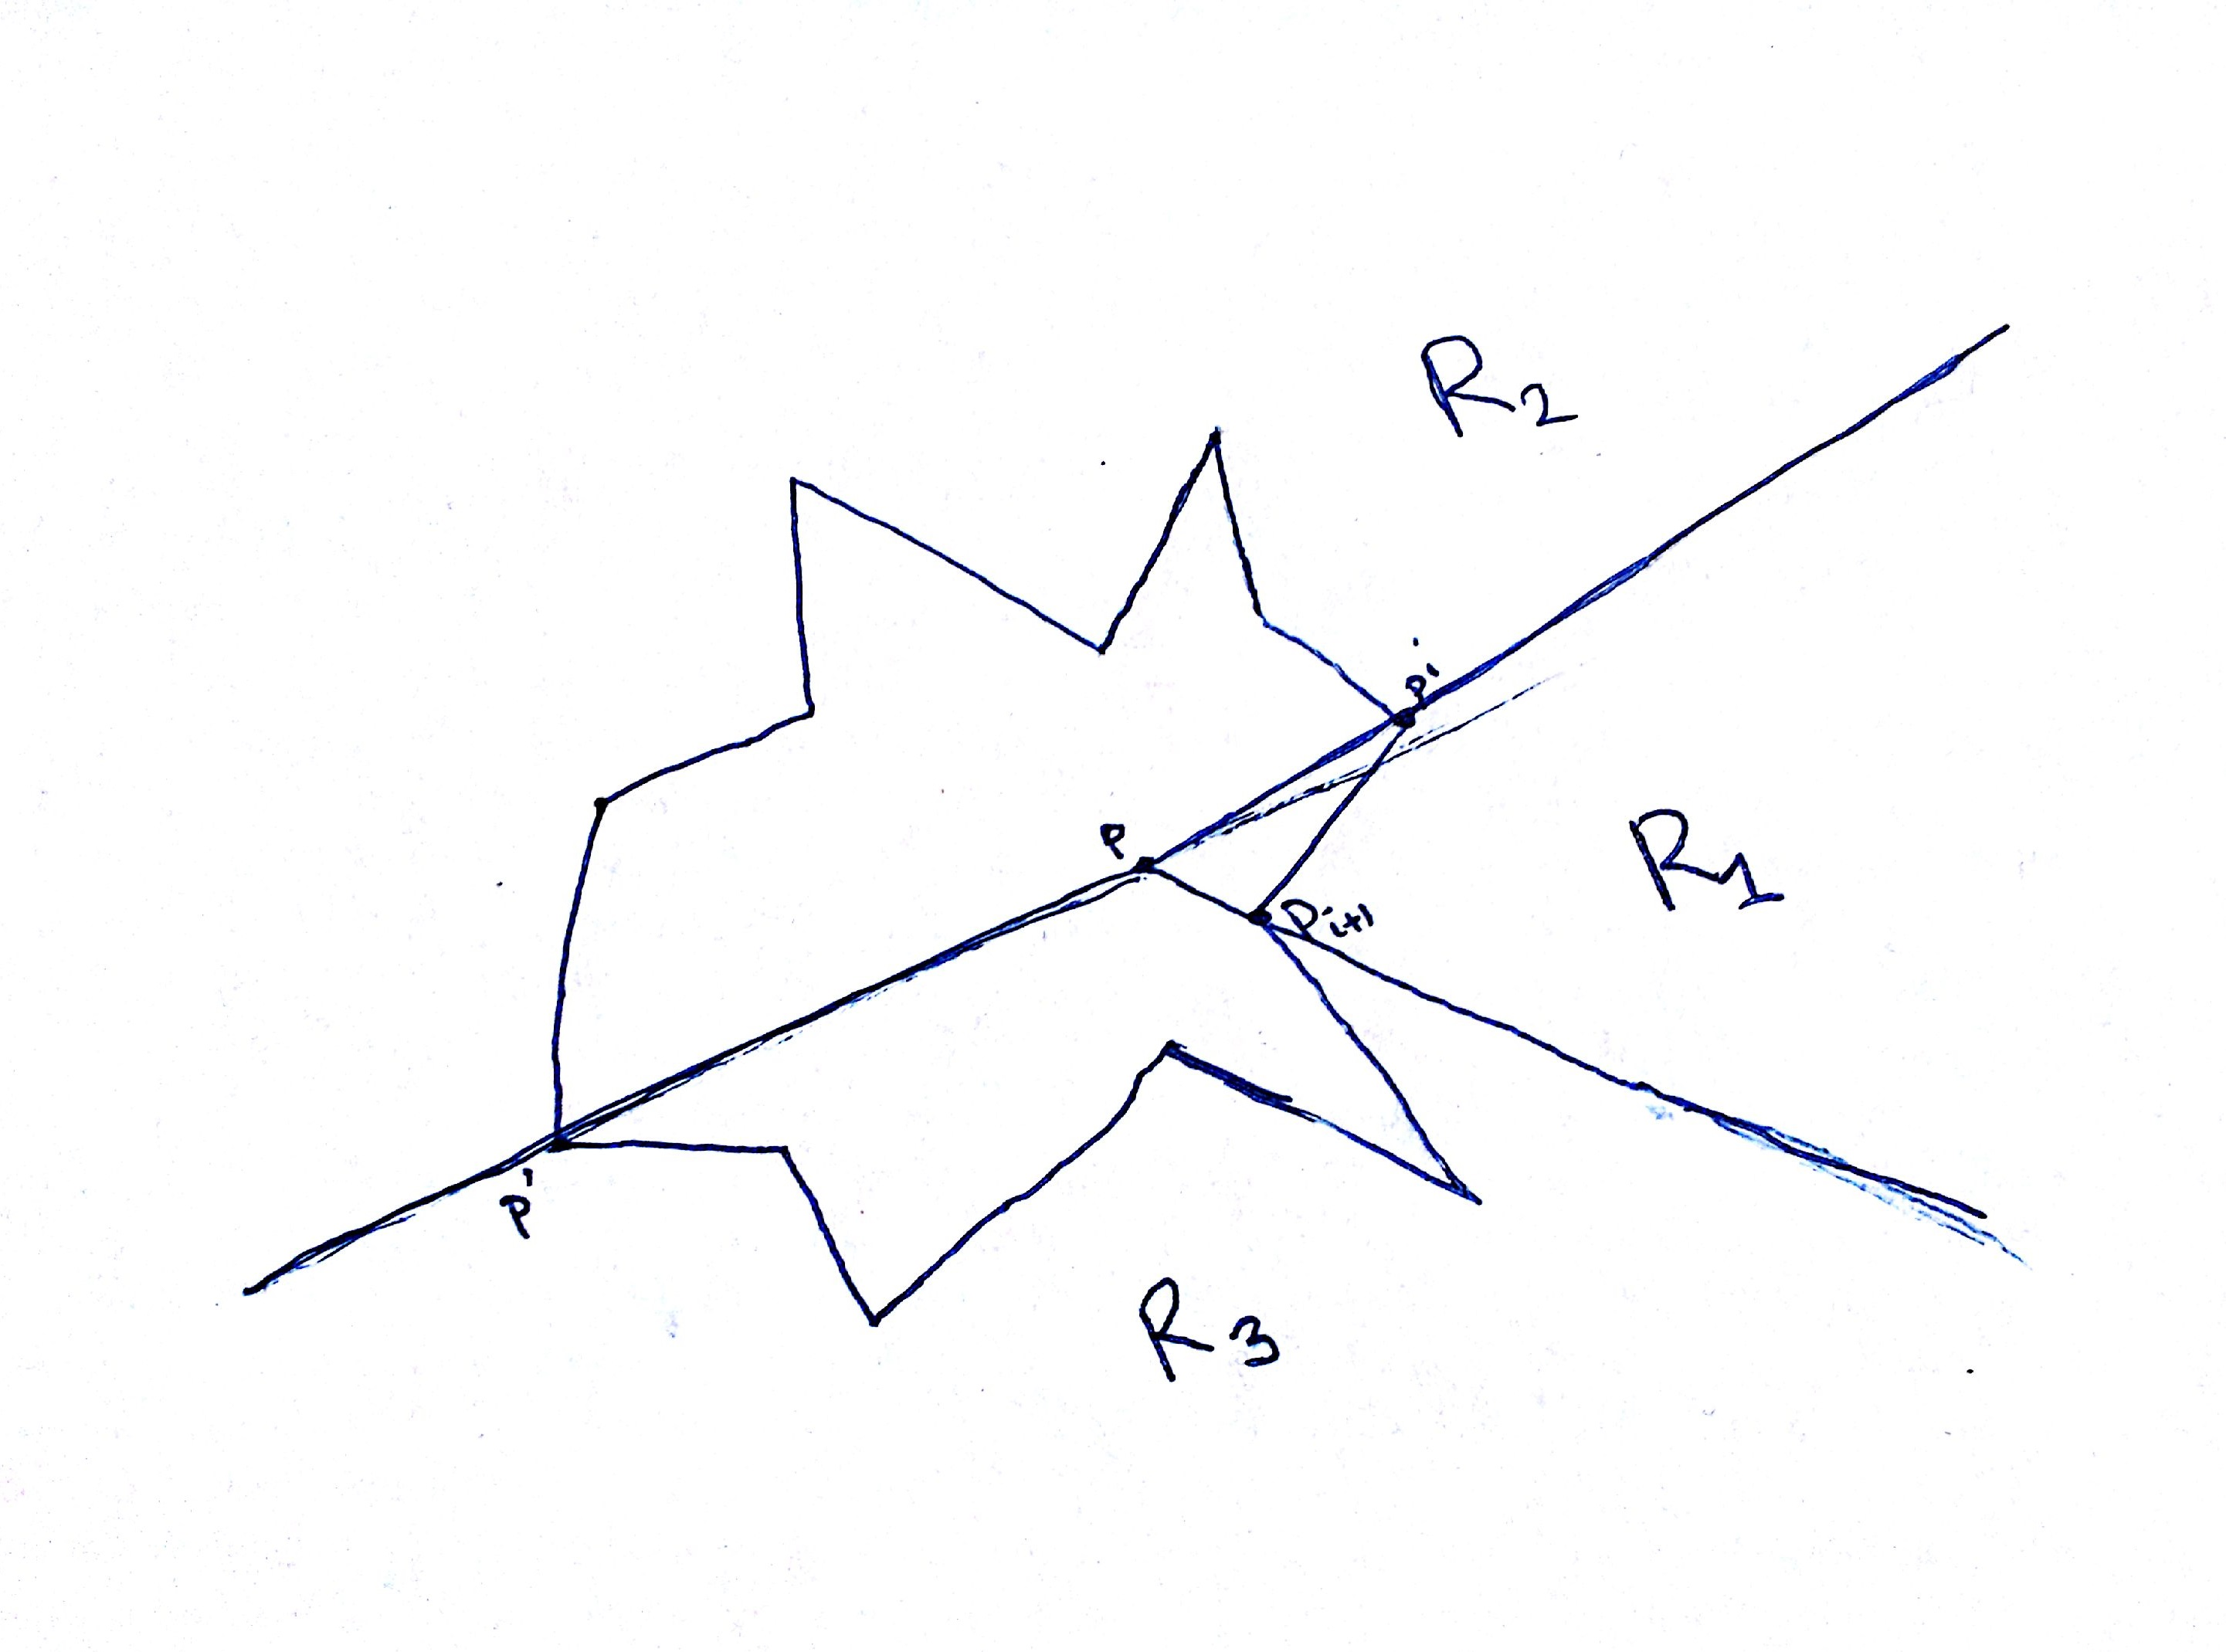
\includegraphics[width=.7\textwidth]{regionsstar2.jpg}
    \caption{The 3 regions, $R1$, $R2$ and $R3$ induced by the half-lines
    from $p$.}
    \label{regions-star}
\end{figure}

In order to determine if $q$ is contained in $P$, we now do as follows:

First, determine which region $q$ is located in; this can be done in constant
time by checking left and right turns from the lines that delimit the
regions.

If $q$ is contained within $R1$, by seeing if the point is
contained within the triangle $p p_i p_{i+1}$.

If $q$ is contained within $R2$, $q$ being contained in $P$ is equivalent to
$q$ being contained in the polygon $p_{i-1} p_i p p' \ldots$.

Using $l = p'$ and $r = p_i$ as start points, we perform a binary search to
narrow down the polygon $p l \ldots r$ around $q$. Once we've reduced the
polygon to a triangle, we can then directly check if the point is contained
within it.

The case for $R3$ is analogous.

\section{Exercise 6.16}

We can use the trapezoidal map from chapter 6 for this
exercise. Corollary 6.4 gives us that we can construct a trapezoidal
map that uses $O(n)$ expected storage in $O(n \log n)$ expected time,
such that the expected point location query time is $O(\log n)$. Upon
finding the face $\delta$ that the query point $q$ belongs to, we can
simply find $top(\delta)$ which will give us the correct line segment.

\end{document}

